
\lesson{29/10}
Making the explicit calculations is not difficult: the derivatives of the
$\vartheta$ simplify for symmetry reasons, so $\slashed{\pd}$ acts only on
the exponentials
$$i\slashed{\pd}_xe^{-ipz} = \slashed{p}e^{-ipz}$$
and the result follows.

\textbf{Note} The Dirac propagator, too, is a Green function of the Dirac operator:
$$(i\slashed{\pd}-m)S_F(x-y)=\delta^4(x-y)$$

\section{Interactions and perturbation Theory}
Until now the Lagrangian of the fields has been free, i.e. without a potential
term: it will now be introduced alongside the kinetic and mass terms.

The interaction term is
$$H_\text{int}:=\int \dd^3x\mathcal{H}_\text{int}(\phi(x^\mu))=-\int \dd^3x
\mathcal{L}_\text{int}(\phi(x^\mu))$$
\textbf{Note} The interaction term is independent of the derivatives of the
field: this is not required, but it is easier to work with, since adding
this dependency would complicate the expression of the conjugate fields.

\textbf{Note} All theories must be \textit{renormalizable}, i.e. the physical
quantities which most of the time turn out to be non-converging integrals must be
tamed: one of the ways is to swap $\infty$ in the extrema of integration with
a "large" parameter $\Lambda$, solve that and hope the result is not dependent on
$\Lambda$; this happens when $\Lambda$ is a dimensionless parameter (e.g. a
coefficient of $\phi^4$ in a scalar interaction).

Other kinds of interaction are the \textit{Yukawa} interaction, which introduces
a term
$$\mathcal{H}_\text{int}=g\bar\phi\psi;$$
and the \textit{electromagnetic interaction} of the QED theory
$$\mathcal{H}_\text{int}= e\bar\psi\gamma^\mu A_\mu\psi.$$
The problem of interacting theories is that \textbf{nothing can be solved exactly
beyond the $\mathbf{\phi^4}$ interaction.}
\subsection{Perturbation in Quantum Mechanics}
The strategy to solve this complex problems is to consider a Hamiltonian with
known solutions, e.g. the free Hamiltonian, and add to it a ``small''
perturbation: these are called \textit{weakly interacting theories}.

Going back to QM, the propagator is
$$K(x_f,x_i,t_f,t_i) = \bra{x_f}U(t_f,t_i)\ket{x_i}$$
and, as is known, it is a Green function $G$ of the Schrödinger operator
$$(E-H)G = \mathbb{I}$$
and so it can be, formally, written as
$$G = \lim\limits_{\varepsilon\to0}\frac{1}{E-H+i\varepsilon} = \frac{1}{E-H_0-V}=
\frac{1}{E-H_0\left(1-\frac{V}{E-H_0}\right)}
$$
In this way, the problem can be expanded in power series via the geometric series
$$G = \frac{1}{E-H_0} \frac{1}{1-\frac{V}{E-H_0}} = G_0\left(1+VG_0+VG_0VG_0
+...\right)$$
where $G_0$ is the propagator of the free Hamiltonian. This is called
\textbf{Dyson series} and can be represented graphically.
\begin{figure}[H]
    \centering
    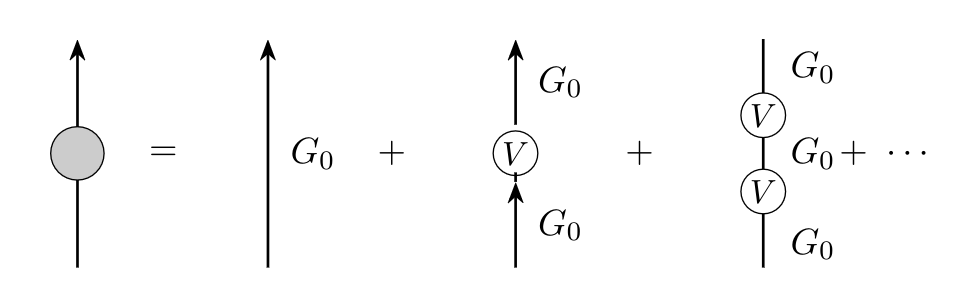
\includegraphics[width = \linewidth]{./prop.png}
\end{figure}
\subsection{Perturbation in QFT}
The free propagator is defined as
$$G_0 = \bra{0}T\phi(x)\phi^\dagger(y)\ket{0}$$
while the most general, interacting propagator is
$$G = \bra{\Omega}T\phi(x)\phi^\dagger(y)\ket{\Omega}$$
where $\ket{\Omega}$ is \textit{the ground state of the interacting system} and
$T$ is the usual time-ordering operator: its interpretation is the same as the
free propagator's with $\ket{\Omega}$ in place of $\ket{0}$.
